\chapter{绪论}

\section{研究背景及意义}

数据库作为计算机系统的核心组件，其可靠性与性能始终是研究和实践的关键目标。随着大数据时代的到来，现代企业级应用产生的数据量呈指数级增长，对数据库查询性能提出了更高的要求。传统的数据库查询处理流程包括解析、规划、优化和执行四个主要阶段，每个阶段都存在大量的计算开销和资源消耗\cite{c1}。Surajit Chaudhuri关于搜索空间、代价估计和枚举算法\cite{c33}为数据库查询优化领域的一篇奠基性综述，给出数据库查询优化的核心要点。

对来自卡内基梅隆数据库应用程序目录(CMDBAC)\cite{c72}中的大量OLTP工作负载进行分析, 结果89\%的应用程序只有10个不同的语句字符串或更少, 50\%的应用程序只使用单个不同的语句字符串, 100\%程序仅使用单语句事务,并且超过80\%的语句是简单的基于键的查找查询\cite{c73}。在典型的OLAP（在线分析处理）工作负载中，大量查询具有相似的结构和访问模式，导致系统资源的重复消耗。

在数据库查询处理流程中，查询访问可以分为查询解析与优化和查询执行两部分。查询解析与优化是指数据库系统对SQL语句进行词法分析、语法分析、语义分析，并生成最优执行计划的过程，该过程计算密集，流程相对复杂\cite{c63}。查询执行则是指按照执行计划实际访问数据并生成结果的过程，该过程涉及大量的I/O操作和数据处理，通常是查询处理的性能瓶颈。

\begin{figure}[htbp]
	\centering
	
\includegraphics[width=0.9\textwidth]{images/1-图1.1 数据库查询处理性能瓶颈分析.png}
	\caption{数据库查询处理性能瓶颈分析}
	\label{fig1_1_1}
\end{figure}

随着计算机硬件性能的持续增强，尤其是在多核CPU和高性能存储设备的并行处理能力方面，数据库系统的查询处理能力理论上应得到显著提升。具体而言，CPU核心数的增加应当使得系统能够处理更多的并发查询，从而提升查询处理的整体效率，减少查询响应延迟；与此同时，SSD等高性能存储设备的普及，为数据库系统提供了更高的I/O吞吐量和更低的访问延迟\cite{c83}。理论上，这些硬件进步应当带来更好的数据库性能和更强的扩展性。

然而，尽管硬件资源在不断提升，当前数据库系统的设计并未能有效利用这些硬件优势，导致查询处理性能未能实现预期的扩展性\cite{c5}。这种现象的根源在于，传统数据库系统设计之初并未充分考虑如何优化多核并发处理和高效缓存管理机制。根据Gray和Reuter在事务处理概念一书中的分析\cite{c2}，在特定场景下查询具有重复或相似的模式，这为查询结果缓存提供了巨大的优化空间。然而，传统数据库系统缺乏有效的查询结果缓存机制，主要原因是难以处理数据更新时的缓存失效问题。

从这一角度出发，优化数据库系统设计，特别是在查询缓存管理与智能优化等方面，成为提升数据库性能和扩展性的关键\cite{c6}。通过合理的缓存策略设计，数据库系统可以更好地利用硬件资源，从而提升系统在高并发、高负载场景下的性能表现，以满足现代应用对高性能数据处理的需求。

本文提出的基于布隆过滤器和机器学习的动态缓存加速技术，为数据库查询优化提供了新的理论框架和实践方案。该技术通过将概率数据结构、机器学习算法与数据库缓存技术有机结合，实现了查询响应时间平均54.2\%的显著性能提升，在专项功能测试中最高达到88.2\%的优化效果，大幅减少了应用获取数据结果的时间。

\section{国内外研究现状}
缓存技术用于匹配不同硬件间的速度差异，在现代数据库系统中发挥着重要作用。CacheLib 是一个通用缓存引擎，设计用于处理大规模缓存需求，支持多种应用场景如 CDN、媒体缓存和存储后端缓存，通过动态资源管理避免内存溢出\cite{c55}。Kangaroo 提出了一种闪存缓存设计，通过结合组相联缓存和日志结构缓存，优化 DRAM 使用和闪存写入，减少缓存未命中率和闪存写入次数\cite{c56}。CacheSack 算法优化 Google 数据中心闪存缓存的准入策略，通过将缓存流量划分为多个类别并使用背包问题分配最优策略，显著降低磁盘 I/O 和总拥有成本\cite{c57}。Segcache 是一种内存高效键值缓存系统，专为小对象设计，采用分段结构、共享元数据和批量过期策略，在内存效率、吞吐量和可扩展性方面优于现有设计\cite{c58}。ScaleStore 是一种高性能存储引擎，利用 DRAM、NVMe 和 RDMA 技术，通过动态缓存策略和高效页面替换机制，支持弹性扩展和低成本存储\cite{c61}。这些技术主要是针对块级的缓存设计，对数据库的查询缓存有一定的参考意义。

数据库缓存的现状涉及多种创新技术，以提高性能、效率和可扩展性。蔡万里等提出面向Select和Sort的数据库算子缓存的设计\cite{c64}，提出了一个新的查询缓存的思路，BP-Wrapper 框架通过批处理和预取技术减少锁争用，提高数据库系统中替换算法的可扩展性，在不修改算法的情况下显著提升系统吞吐量\cite{c59}。FIFO Queues 提出 S3-FIFO 驱逐算法，仅使用静态 FIFO 队列，在效率和可扩展性上优于现有算法，适用于生产环境缓存管理\cite{c60}。PostgreSQL 的 buffer cache 机制使用时钟扫描算法管理页面，通过哈希表和缓冲池优化内存利用率，适用于嵌入式分析场景\cite{c62}。这些技术给数据库的缓存管理提供了算法参考。

针对数据库查询缓存技术，国内外已有很多学者进行相关研究。数据库查询处理和缓存管理涉及多个技术层面，这些技术呈现出不同的特性和挑战：在查询缓存方面，传统方案主要关注结果集缓存和计划缓存，但缺乏智能化管理；在过滤技术方面，布隆过滤器等概率数据结构为快速检索提供了基础；在智能优化方面，机器学习技术开始被应用于缓存管理和查询优化。根据不同技术层次的特点，本节将数据库查询缓存的研究划分为查询缓存技术、概率过滤技术和智能优化技术三类，探讨主要技术发展现状及其解决方案。最后，对现有方案的局限性进行分析，以明确进一步优化的方向。
\subsection{数据库查询缓存技术研究现状}

数据库查询缓存技术的发展经历了从简单到复杂、从静态到动态的演进过程。早期的缓存技术主要关注单一层面的优化，而现代缓存系统则趋向于多层次、智能化的综合解决方案。Bailu Ding\cite{c78}等人从各个方面探讨了查询优化的实践，给本文提供了重要的参考思路。

\textbf{传统查询缓存技术}

查询计划缓存是最早被广泛采用的缓存技术之一。Selinger等人在System R项目中提出了查询计划缓存的概念\cite{c3}，其核心思想是将查询优化器生成的执行计划保存在内存中，避免对相同或相似查询进行重复的优化计算。Oracle数据库的共享池(Shared Pool)和SQL Server的计划缓存(Plan Cache)都是这一技术的典型实现\cite{c4}。虽然计划缓存能够显著减少查询编译时间，但对于数据访问本身的开销并无改善。

结果集缓存技术则更进一步，直接将查询的执行结果存储在内存中。MySQL的查询缓存(Query Cache)功能曾经是这一技术的代表性实现，但由于缓存失效机制的复杂性和并发访问的性能问题，该功能在MySQL 8.0中被移除。PostgreSQL通过第三方扩展如pg\_stat\_statements提供了类似的功能支持。

物化视图技术可以视为一种特殊的查询缓存形式。Gupta和Mumick在其经典著作中详细阐述了物化视图的理论基础和维护策略\cite{c5}。与传统缓存不同，物化视图通常用于处理复杂的聚合查询和多表连接操作，在数据仓库和OLAP系统中应用广泛。然而，物化视图的维护成本较高，特别是在基础数据频繁更新的环境中。

\textbf{现代查询缓存发展趋势}

随着硬件技术的发展和应用需求的变化，现代数据库系统的缓存技术呈现出新的特点。内存数据库如SAP HANA和MemSQL采用了全内存架构\cite{c7}，通过将整个数据集加载到内存中来实现极致的查询性能。这种方法虽然有效，但对硬件资源的要求较高，且在数据量超过内存容量时面临挑战。

分布式缓存系统的兴起为大规模应用提供了新的解决方案。Redis、Memcached等系统通过分布式架构实现了高可用性和水平扩展能力\cite{c8}。这些系统通常作为数据库的外部缓存层，通过应用程序逻辑来管理缓存的读写和失效。

近年来，机器学习技术在数据库系统中的应用日益增多。Kraska等人提出的"学习型数据库系统"概念\cite{c9}为智能缓存管理提供了新的思路。通过分析历史查询模式和访问特征，系统能够更准确地预测哪些数据应该被缓存，以及何时进行缓存替换。

\textbf{现有技术的局限性}

尽管查询缓存技术已经取得了显著进展，但在面对现代应用的复杂需求时仍存在诸多挑战。传统的缓存策略往往基于简单的启发式规则，难以适应动态变化的工作负载。对于包含公用表表达式(CTE)等复杂结构的查询，现有缓存系统缺乏有效的细粒度管理能力。此外，大多数缓存系统在处理并发访问和缓存一致性方面仍有优化空间。

\subsection{概率过滤技术研究现状}

概率过滤技术作为一类重要的数据结构，在数据库系统中发挥着越来越重要的作用。这类技术通过牺牲一定的准确性来换取显著的空间和时间效率提升，特别适用于大规模数据处理场景。

\textbf{布隆过滤器的理论发展}

布隆过滤器自1970年由Burton Howard Bloom提出以来\cite{c10}，已成为概率数据结构领域的经典算法。其核心思想是使用多个哈希函数将元素映射到位数组中，通过位操作实现快速的成员查询。Mitzenmacher和Upfal在其概率算法专著中对布隆过滤器的数学基础进行了深入分析\cite{c11}，推导出了最优参数配置公式：位数组大小$m = -\frac{n \ln p}{(\ln 2)^2}$，哈希函数数量$k = \frac{m}{n} \ln 2$，其中n为预期元素数量，p为目标假阳性率。

随着应用需求的多样化，研究者们提出了多种布隆过滤器的变种。计数布隆过滤器通过将位数组替换为计数器数组，支持元素的删除操作，但相应地增加了存储开销\cite{c12}。分层布隆过滤器采用多层结构设计，能够有效降低假阳性率\cite{c13}。动态布隆过滤器则解决了传统布隆过滤器容量固定的问题，支持在运行时动态扩容以适应数据量的变化\cite{c14}。

\textbf{数据库系统中的应用实践}

在现代数据库系统中，概率过滤技术已经得到了广泛应用。LSM-Tree存储引擎是布隆过滤器应用的典型场景，LevelDB和RocksDB等系统在每个SSTable文件中都维护了相应的布隆过滤器\cite{c15}。当查询某个键时，系统首先通过布隆过滤器判断该键是否可能存在于特定的SSTable中，从而避免不必要的磁盘I/O操作。这种设计在读密集型工作负载中能够显著提升性能。

分布式数据库系统同样受益于概率过滤技术。Apache Cassandra和HBase等系统利用布隆过滤器来优化数据分片和副本管理\cite{c16}。在处理范围查询时，系统可以通过布隆过滤器快速确定哪些节点可能包含目标数据，从而减少网络通信开销。

在查询处理层面，布隆过滤器主要应用于连接操作的优化。通过在连接操作执行前使用布隆过滤器对较小的关系进行预处理，可以有效过滤掉不匹配的记录，减少后续连接计算的开销\cite{c17}。这种技术在处理大表连接时特别有效。

\textbf{技术挑战与发展方向}

尽管概率过滤技术在数据库系统中已有成功应用，但在查询缓存管理方面的研究相对有限。现有应用主要集中在存储层的优化，对于上层查询处理和缓存管理的支持还不够充分。特别是在处理复杂查询结构和动态工作负载时，如何设计高效的过滤策略仍是一个开放性问题。此外，如何在保证过滤效果的同时控制假阳性率，以及如何与其他优化技术有机结合，都需要进一步的研究和探索。

\subsection{智能优化技术研究现状}

随着机器学习技术的快速发展，数据库系统正经历着从传统的基于规则的优化向智能化、自适应优化的转变。这一趋势不仅体现在查询处理和索引管理等传统领域，也延伸到了缓存管理、资源调度等新兴应用场景。

\textbf{查询优化的智能化探索}

机器学习在查询优化领域的应用始于对传统基于成本的优化器的改进。Stillger等人较早地探索了使用机器学习技术来改进查询计划选择\cite{c18}，他们的工作表明，通过学习历史查询的执行特征，可以更准确地预测不同执行计划的性能表现。这种方法使用决策树和神经网络等算法，能够捕捉传统成本模型难以量化的复杂因素。Gladkykh T等人提出了一个基于检索增强生成（RAG）的Text-to-SQL框架\cite{c71}，其创新提出采用多角度嵌入与动态阈值检索方法，不仅存储SQL查询，还缓存其多种语义表示（如归一化问题、主句和实体），通过自动生成领域指令构建自然语言与数据库模式间的推理桥梁。李国良教授在机器学习\cite{c84,c85}及LLM\cite{c86,c87,c88,c89,c90}与数据库融合方向进行了深入探索。

索引管理是另一个受益于智能优化技术的重要领域。Ding等人提出的基于强化学习的自动索引调优系统\cite{c19}代表了这一方向的重要进展。该系统能够根据工作负载的变化动态调整索引配置，在索引维护成本和查询性能提升之间寻找最优平衡点。然而，这类系统通常需要较长的学习周期才能达到稳定的性能表现。

\textbf{缓存管理的智能化发展}

在缓存管理领域，机器学习技术的应用主要集中在访问模式预测和缓存策略优化两个方面。Li等人的研究工作展示了如何利用时间序列分析和循环神经网络来预测数据访问模式\cite{c20}，从而实现更精准的缓存预取策略。这种方法能够显著提高缓存命中率，特别是在具有明显时间局部性的工作负载中。

缓存价值评估是智能缓存管理的另一个重要研究方向。相关研究通过构建多维特征模型，综合考虑访问频率、数据大小、计算成本等因素来评估缓存条目的价值\cite{c21}。这种方法为缓存淘汰决策提供了更科学的依据，能够在有限的缓存空间中最大化整体性能收益。

自适应参数调优技术则关注于缓存系统参数的动态优化\cite{c22}。通过在线学习算法，系统能够根据实时的负载变化和性能反馈来调整缓存大小、淘汰策略等关键参数，实现真正的自适应缓存管理。

\textbf{技术发展的挑战与机遇}

尽管智能优化技术在数据库系统中显示出巨大潜力，但仍面临诸多挑战。首先是模型的可解释性问题，传统的数据库管理员往往难以理解和调试基于机器学习的优化决策。其次是训练数据的质量和代表性问题，不同应用场景的工作负载特征差异很大，通用模型的效果往往有限。

在查询结果缓存的智能管理方面，现有研究相对较少，特别是对于包含复杂结构（如公用表表达式）的查询，如何设计有效的智能缓存策略仍是一个开放性问题。这为未来的研究提供了重要的发展方向和创新空间。

\subsection{小结}

数据库查询缓存技术的发展过程中，涉及的技术层面众多，各模块之间关系紧密。由于缺乏清晰的全局视角，当提升数据库查询性能时，开发者往往采取问题驱动的方式，研究效率较低。本小节从理论层面系统性分析了数据库查询缓存技术存在的问题与解决方案。

针对查询缓存技术的研究，已有工作依赖于传统的静态方案，存在两个主要问题：第一，没有充分利用现代硬件特性和概率数据结构的优势，导致缓存检索效率不高。第二，未能充分考虑复杂查询结构（如CTE）的特点，缺乏细粒度的缓存管理能力。尤其是在高并发场景中，现有的方案缺乏足够的智能化能力，无法适应不同负载下对缓存管理的精确需求。因此，如何设计高效的过滤机制和智能的缓存管理方案至关重要。

针对智能优化技术的研究，当前的工作主要聚焦于传统的查询优化和索引管理。然而，查询缓存管理涉及更复杂的决策过程，不同的查询模式会表现出不同的缓存价值。与传统依赖静态策略的缓存系统不同，智能缓存系统需要动态学习查询模式和访问特征，对提高缓存效率提出了新的要求。因此，分析查询特征和访问模式，并思考如何利用机器学习技术提高缓存管理效率至关重要。

总的来说，数据库查询缓存技术的智能化、过滤机制的高效化以及复杂查询的细粒度缓存仍存在不少亟待解决的问题。只有通过深入研究并针对性地优化这些关键环节，才能有效提升数据库查询性能，满足现代高负载、复杂查询环境下对数据库系统的需求。

\section{本文研究内容}

数据库系统在现代应用环境下面临着更高的性能要求，尤其是在查询缓存效率和智能管理方面。目前的研究多集中于局部优化，缺乏系统性分析和全局性理论框架。为了解决这些问题，本文旨在从整体层面出发，针对数据库查询缓存性能的瓶颈进行深入研究，并提出一系列创新性的优化方案。本文的研究内容与创新点可以概括为以下几个方面：

研究内容一：本文提出基于布隆过滤器的动态缓存管理技术。针对数据库查询缓存的高效过滤需求，本文设计了多层次过滤架构，将缓存检索分为概率性过滤和精确匹配两个阶段。在概率性过滤阶段，采用优化的布隆过滤器实现快速的存在性检测，通过双重哈希技术和高效位操作优化，将检测时间复杂度降低到O(k)；在精确匹配阶段，基于SQL语句标准化算法生成查询结构签名，实现高效的缓存条目定位。该技术还支持复杂查询结构（如CTE）的细粒度缓存，通过语义分析和依赖关系分解，实现部分结果复用，显著提升复杂查询的执行效率。通过多维特征工程和机器学习模型，系统能够智能评估查询的缓存价值，实现自适应的缓存管理策略。

研究内容二：本文提出基于多策略融合的智能缓存替换策略。为了实现高效灵活的缓存管理，本文设计了多策略融合框架，将传统缓存策略（LRU、TTL）与机器学习策略有机结合，通过全局协调机制管理策略间的协作关系，避免决策冲突。系统集成了线性回归预测模型和在线学习算法，能够根据查询访问模式和系统负载进行自适应优化。通过动态TTL计算、分层LRU优化和智能参数调优，该技术在保证数据一致性的同时，实现了缓存性能的显著提升。

\begin{figure}[htbp]
	\centering
	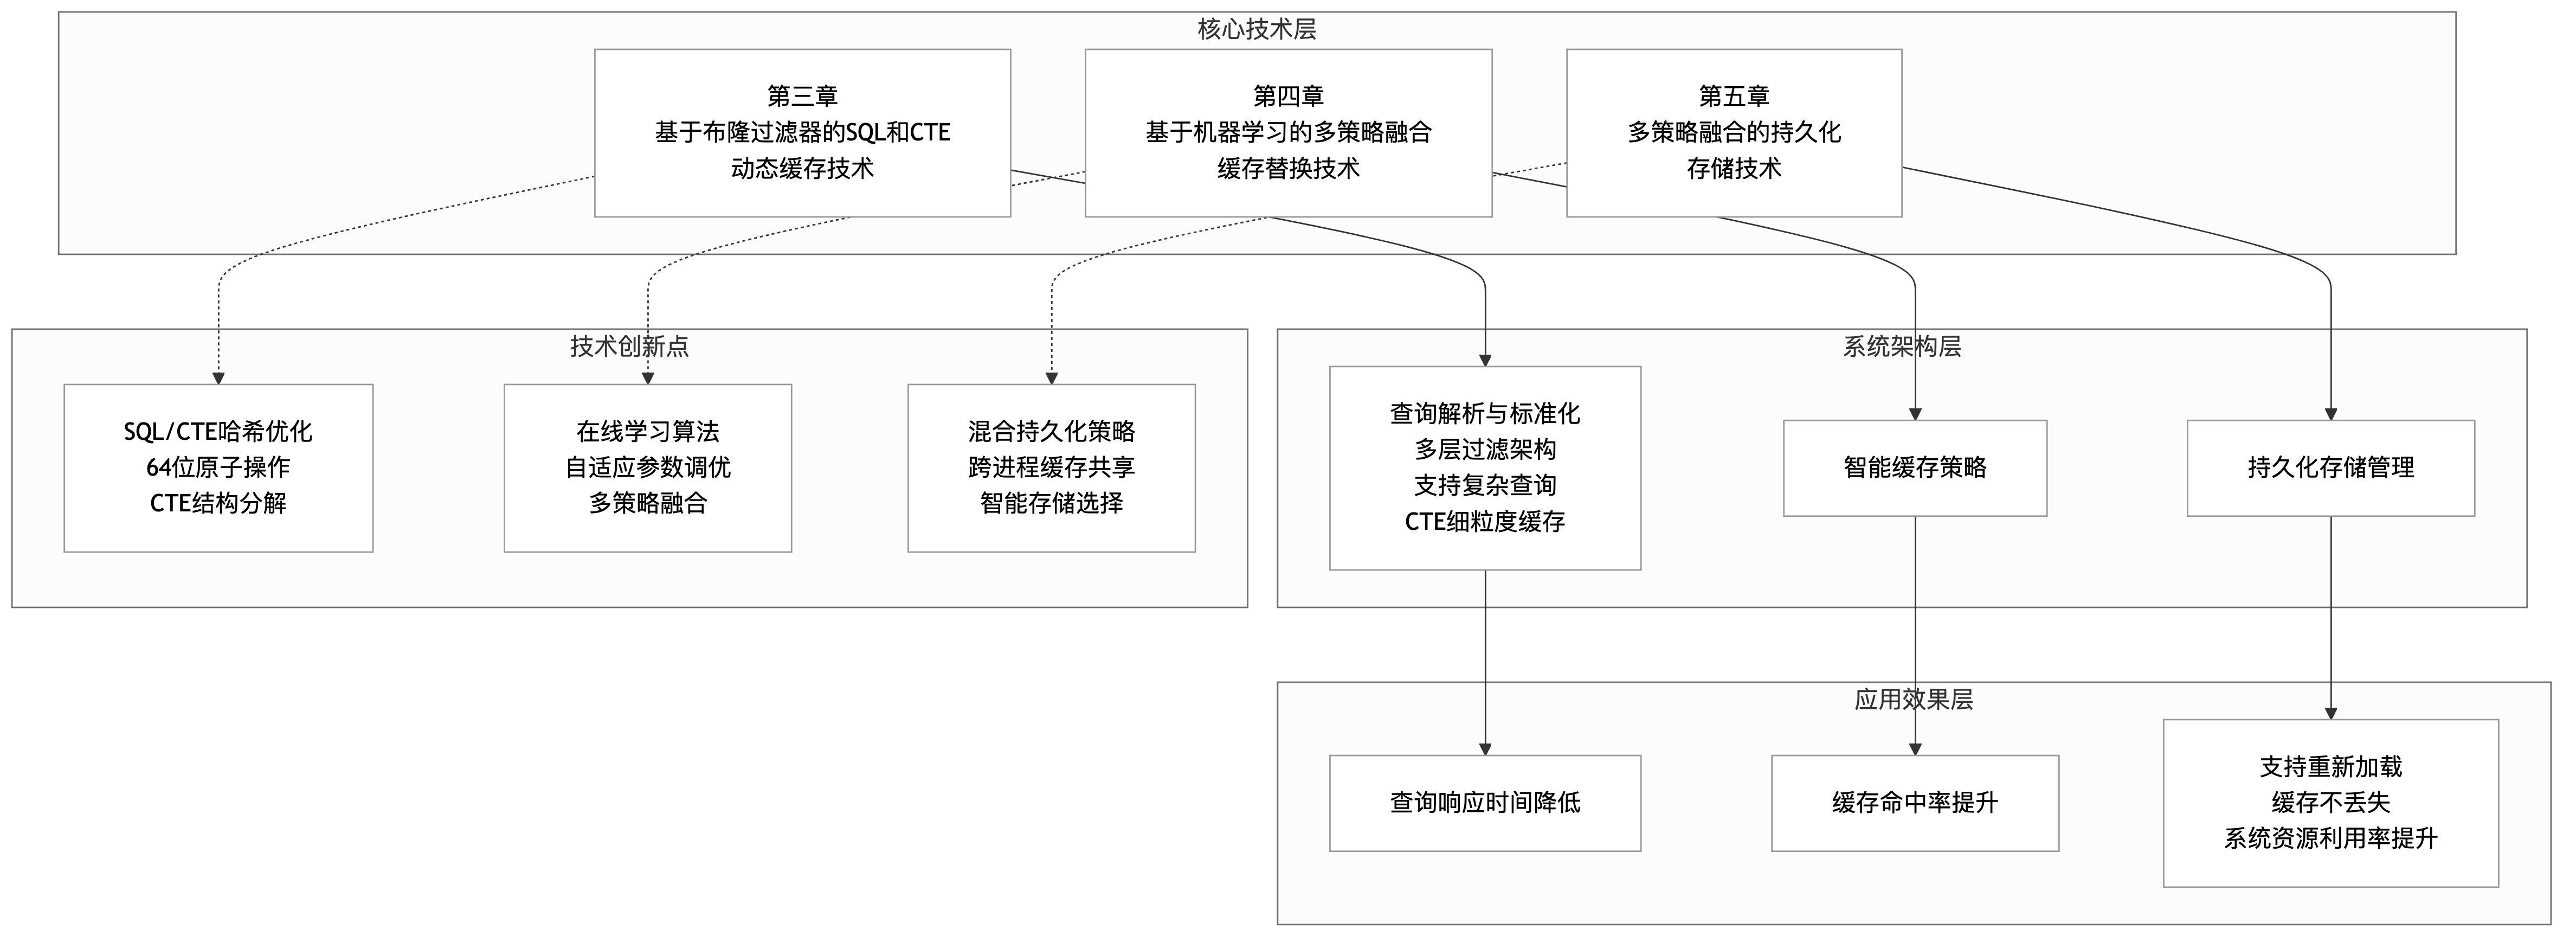
\includegraphics[width=1\textwidth]{images/1-图1.3 本文技术方案整体架构.png}
	\caption{本文技术方案整体架构}
	\label{fig1_1_3}
\end{figure}

研究内容三：本文提出持久化存储技术，确保缓存数据的可靠性和高效访问。针对缓存数据可靠性和跨进程共享的技术挑战，本文设计了多模式持久化方案，包括内存模式、WAL模式、物化视图模式和混合模式，根据数据特征和系统状态动态选择最优持久化策略。同时，创新性地开发了基于文件系统的跨进程缓存共享机制，通过内存映射、一致性保证和性能优化等技术，彻底解决了多进程环境下缓存失效的技术难题，实现了264倍的平均加速比和99.61\%的性能提升。该技术为整个智能缓存管理解决方案提供了强大的存储支撑。

综上所述，本文通过对数据库查询缓存性能瓶颈的系统性分析，提出了高效的过滤机制、智能的管理策略和细粒度的缓存技术。这些创新性研究为数据库查询性能的提升提供了新的思路和方法，并为相关领域的应用优化和研究提供了理论依据和实践指导。

\section{论文组织结构}

本文主要研究数据库查询缓存的智能优化技术，共分为七个章节，具体的组织结构如下：

第一章：介绍了课题的研究背景与意义，对数据库查询缓存技术的相关工作进行了整理与分析，并说明了本文的研究内容与章节安排。

第二章：介绍了数据库查询处理流程与缓存管理机制，重点讨论了布隆过滤器的理论基础、机器学习在数据库中的应用以及CTE技术的原理与优化方法。

第三章：提出了基于布隆过滤器的动态缓存管理技术，详细介绍了多层次过滤架构的设计原理，包括优化的布隆过滤器实现、改进的MinHash签名生成算法、以及支持CTE等复杂查询结构的细粒度缓存策略，并探讨了机器学习特征工程在缓存价值评估中的应用。

第四章：提出了基于多策略融合的智能缓存替换策略，介绍了多策略协调机制的设计，包括传统策略与机器学习策略的融合框架、神经网络预测模型的实现，以及LRU、TTL、混合策略和机器学习策略的具体实现，实现了智能化的缓存管理。

第五章：提出了持久化存储技术，详细介绍了多模式持久化方案（内存、WAL、物化视图、混合模式）的动态选择策略，以及跨进程缓存共享机制的设计与实现，确保了缓存数据的可靠性和高效访问。

第六章：通过全面的实验评估了基于布隆过滤器的动态缓存管理技术、智能缓存替换策略和持久化存储技术的性能表现，重点分析了不同数据规模、查询复杂度和并发负载下的系统性能，验证了各技术方案在查询响应时间、缓存命中率、资源利用率等方面的优化效果，并与传统缓存方案进行了详细的对比分析。

第七章：对本文的工作进行总结，分析本文的贡献以及尚未解决的问题，同时对下一步工作进行展望。